\documentclass[conference]{IEEEtran}
\usepackage{cite}
\usepackage{amsmath,amssymb,amsfonts}
\usepackage{graphicx}
\usepackage{textcomp}
\usepackage{xcolor}
\usepackage{booktabs}
\usepackage{tikz}
\usetikzlibrary{arrows.meta,positioning,shapes.geometric,fit}
\usepackage{url}
\usepackage{array}
\usepackage{algorithm}
\usepackage{algorithmic}

\def\BibTeX{{\rm B\kern-.05em{\sc i\kern-.025em b}\kern-.08em
    T\kern-.1667em\lower.7ex\hbox{E}\kern-.125emX}}

\begin{document}

\title{Agentic AI for Plant Disease Diagnosis: An Autonomous Multi-Agent Framework Integrating Vision, Retrieval, and Reasoning}

\author{
\IEEEauthorblockN{Lovepreet Sharma}
\IEEEauthorblockA{Department of Information Technology \\
Dr BR Ambedkar National Institute of Technology \\
Jalandhar, Punjab, India \\
lovepreets.da.25@nitj.ac.in}
\and
\IEEEauthorblockN{Mithilesh Tiwari}
\IEEEauthorblockA{Department of Information Technology \\
Dr BR Ambedkar National Institute of Technology \\
Jalandhar, Punjab, India \\
mithlisht.da.25@nitj.ac.in}
\and
\IEEEauthorblockN{Dr. Jaspal Kaur Saini}
\IEEEauthorblockA{Department of Information Technology \\
Dr BR Ambedkar National Institute of Technology \\
Jalandhar, Punjab, India \\
{}saini@nitj.ac.in}
}

\maketitle

\begin{abstract}
Automated plant disease detection using convolutional neural networks has achieved strong classification accuracy on benchmark datasets such as PlantVillage, yet a standalone classifier provides only a label and a confidence score: it offers no explanation, no differential reasoning over plausible alternatives, and no mechanism to defer uncertain cases to a human expert. This paper presents an agentic artificial intelligence framework that wraps a ResNet-18 vision classifier with four cooperating agents -- a Confidence and Image-Quality Agent, a Retrieval Agent, a Reasoning Agent, and an Orchestrator -- to convert disease classification into an autonomous, explainable, and safety-aware diagnostic advisory system. The Orchestrator conditions expensive retrieval and reasoning computation on prediction confidence and class ambiguity, invoking a full retrieval-augmented reasoning pipeline only for uncertain cases and escalating low-confidence, low-quality inputs directly to human review rather than acting on them. We evaluate the system on the PlantVillage dataset using both conventional classification metrics and a set of agentic metrics -- correct-action rate, harmful-action rate, and human-intervention rate -- that quantify the safety-utility trade-off of autonomous deferral relative to a naive always-trust-the-classifier baseline. On a held-out test set of 114 images spanning all 38 classes, a single ResNet-18 classifier attains a top-1 accuracy of 86.0\%, and the agentic layer reduces the harmful-action rate from a naive always-act baseline of 14.0\% to 3.5\%, at a human-intervention rate of 17.5\%. Replacing the single backbone with a three-model federated ensemble (FedAvg, FedOpt, FedMA) further raises classification accuracy on this in-distribution split and supplies an inter-model agreement signal to the Orchestrator. These results support agent-orchestrated pipelines as a practical bridge between high-accuracy vision models and trustworthy, deployable agricultural decision support.
\end{abstract}

\begin{IEEEkeywords}
Agentic AI, Plant Disease Detection, Retrieval-Augmented Generation, Multi-Agent Systems, PlantVillage, ResNet-18, Precision Agriculture, Autonomous Decision-Making
\end{IEEEkeywords}

\section{Introduction}
\label{sec:intro}

Plant diseases remain among the largest threats to global food security, with crop losses attributable to pests and pathogens estimated to reduce yields by 20--40\% annually across major staple crops. Early and accurate diagnosis is the single most effective lever for limiting this loss, since most fungicide and cultural interventions are far more effective when applied before a disease reaches an advanced stage. The introduction of large, labeled image datasets such as PlantVillage \cite{r_hughes2015}, together with deep convolutional architectures, has made it possible to train classifiers that recognize dozens of crop-disease categories from a single leaf photograph with accuracy exceeding 95\% on held-out benchmark data \cite{r_mohanty2016}.

Despite this accuracy, a bare classifier is a narrow, reactive tool in the sense described by the broader agentic AI literature \cite{b1,b9}: it consumes an image and returns a label and a softmax score, with no capacity to explain \emph{why} a diagnosis was reached, no mechanism to weigh alternative diagnoses when the image is ambiguous, and -- most critically for a system whose output may drive real pesticide use -- no way to recognize its own uncertainty and defer to a human expert. A classifier that is wrong 5\% of the time will, if deployed naively, confidently recommend the wrong treatment in exactly those 5\% of cases, with no distinguishing signal to separate them from the 95\% it gets right.

Agentic artificial intelligence -- systems characterized by autonomy, goal-directed behavior, tool use, and the capacity to plan multi-step actions in response to their environment -- has been proposed as a paradigm for exactly this class of problem across domains such as healthcare, energy management, and climate modeling \cite{b1,b3,b6,b13,b14}. Reviews of agentic AI applications have surveyed its use extensively in these areas \cite{b2,b5,b10}, yet its application to agricultural disease diagnosis as an autonomous, safety-aware decision-support agent has received comparatively little attention. Existing plant-disease work overwhelmingly frames the problem as pure image classification, leaving the reasoning, retrieval, and deferral behavior that would make such a system trustworthy for real-world deployment largely unaddressed.

This paper closes that gap. We present an agentic architecture that reuses a trained plant-disease classifier as a perception module and wraps it with four cooperating agents that together transform a single-shot classification into an autonomous diagnostic workflow. The specific contributions of this paper are:

\begin{enumerate}
\item We propose and implement a five-component agentic architecture -- Vision, Confidence/Quality, Retrieval, Reasoning, and Orchestrator -- that upgrades a standard CNN plant-disease classifier into an autonomous diagnostic advisory agent.
\item We design an orchestration policy that conditions retrieval and reasoning computation on prediction confidence and class ambiguity, so that computationally expensive reasoning is invoked only where it is needed, while low-confidence or low-quality inputs are escalated to a human rather than acted upon.
\item We introduce a set of agentic evaluation metrics -- correct-action rate, harmful-action rate, and human-intervention rate -- that capture the safety-utility trade-off of an autonomous diagnostic system in a way that classification accuracy alone cannot.
\item We report an empirical evaluation of the complete pipeline on the PlantVillage benchmark, quantifying the reduction in harmful-action rate achieved relative to a naive classifier-only baseline.
\end{enumerate}

The remainder of this paper is organized as follows. Section~\ref{sec:related} reviews the foundations of agentic AI and positions this work relative to prior plant-disease classification research. Section~\ref{sec:arch} describes the proposed multi-agent architecture. Section~\ref{sec:impl} details the implementation. Section~\ref{sec:exp} defines the experimental protocol and metrics. Section~\ref{sec:results} reports results, and Section~\ref{sec:conclusion} concludes with directions for future work.

\section{Related Work}
\label{sec:related}

\subsection{Foundations of Agentic AI}
Agentic AI refers to systems designed with autonomy, goal-directed behavior, and the capacity to take initiative, moving beyond passive tools that only respond to prompts \cite{b1,b9}. Four capabilities are commonly identified as its foundation. \emph{Reinforcement learning} provides a framework for sequential decision-making under reward and penalty, prioritizing experiential learning over supervised label-fitting \cite{r1}. \emph{Goal-oriented architectures} give an agent explicit objectives against which it can plan and prioritize actions, integrating symbolic reasoning and planning with learned components \cite{r2,b11}. \emph{Autonomous decision-making} is the capacity to evaluate options and act without continuous human supervision, underpinned by perception, reasoning, and action-selection mechanisms \cite{b12}. \emph{Environment interaction} closes the loop: an agent perceives state, updates an internal model, and takes actions that alter its environment, enabling adaptation to conditions that were not seen during training \cite{b4}.

A closely related concept is agentic memory, commonly decomposed into procedural, short-term, long-term, episodic, and semantic memory \cite{b1}. Procedural memory stores reusable action sequences; short-term memory holds task-local context; long-term and semantic memory persist facts and preferences across sessions; and episodic memory records specific past interactions to inform future behavior. As detailed in Section~\ref{sec:arch}, the present system deliberately implements only the semantic-memory component required for retrieval-augmented reasoning, treating persistent episodic memory and longitudinal disease tracking as a scoped future extension (Section~\ref{sec:conclusion}) rather than a claim made in the current implementation.

\subsection{Traditional versus Agentic AI}
Table~\ref{tab:comparison} summarizes the distinction between the traditional classification paradigm that dominates existing plant-disease literature and the agentic paradigm adopted in this work. The key shift is from a system that is reactive and provides a single output, to one that is proactive, reasons over multiple candidate outcomes, and can decline to act.

\begin{table}[t]
\centering
\caption{Traditional AI versus Agentic AI}
\label{tab:comparison}
\small
\begin{tabular}{p{1.6cm}p{2.7cm}p{2.9cm}}
\toprule
\textbf{Aspect} & \textbf{Traditional AI} & \textbf{Agentic AI (this work)} \\
\midrule
Output & Label + confidence score & Diagnosis, grounded explanation, treatment, and a deferral decision \\
Initiative & Reactive; always emits a prediction & Proactive; may withhold action and request human review \\
Reasoning & Single forward pass & Multi-step: perceive, assess, retrieve, reason, act \\
Uncertainty handling & None; wrong predictions are indistinguishable from correct ones & Explicit confidence and ambiguity gating via the Orchestrator \\
Explanation & None & Retrieved-passage-grounded justification \\
\bottomrule
\end{tabular}
\end{table}

\subsection{Deep Learning for Plant Disease Detection}
The PlantVillage dataset \cite{r_hughes2015} and the benchmark results of Mohanty et al.\ \cite{r_mohanty2016} established convolutional neural networks as the dominant approach for image-based plant disease diagnosis, with subsequent work exploring deeper backbones, transfer learning, and federated training across distributed agricultural data sources. This body of work optimizes exclusively for classification accuracy; none of it, to our knowledge, addresses the downstream question of \emph{what an automated system should do} with a prediction once it is made -- whether to act on it, explain it, or defer it -- which is the problem this paper addresses.

\subsection{Agentic AI in Agriculture}
Surveys of agentic AI applications have covered healthcare \cite{b11,b1}, finance, cybersecurity, and climate and energy management in considerable depth \cite{b2,b6,b13}, documenting autonomous agents that monitor, plan, and act with limited human oversight in each of these domains. Agriculture is frequently listed as a target domain for agentic AI in these broader surveys, typically in connection with resource optimization, irrigation scheduling, or supply-chain management at the farm or regional level. However, at the level of an individual diagnostic interaction between a farmer, a leaf photograph, and a recommended treatment, the literature remains dominated by single-model image classifiers. The architecture proposed in this paper is, to our knowledge, among the first to apply the full agentic pattern -- perception, uncertainty-aware reasoning, tool-augmented retrieval, and autonomous deferral -- to this specific and consequential diagnostic setting, where an incorrect autonomous recommendation carries a direct economic and food-security cost.

\subsection{Retrieval-Augmented Generation}
Retrieval-augmented generation (RAG) couples a language model with a non-parametric retrieval step over an external corpus, grounding generated text in retrieved evidence rather than relying solely on parametric knowledge \cite{r_lewis2020}. This mechanism is well suited to diagnostic explanation, where the treatment and prevention advice given to a farmer should be traceable to an authoritative agricultural source rather than generated from the language model's unverified prior knowledge. Section~\ref{sec:arch} describes how this work employs RAG as the semantic-memory substrate for the Reasoning Agent.

\section{Proposed System Architecture}
\label{sec:arch}

The system is composed of five cooperating components: a Vision Agent, a Confidence and Image-Quality Agent, a Retrieval Agent, a Reasoning Agent, and an Orchestrator that governs control flow between them. Fig.~\ref{fig:arch} illustrates the architecture and the two execution paths the Orchestrator can select.

\begin{figure}[t]
\centering
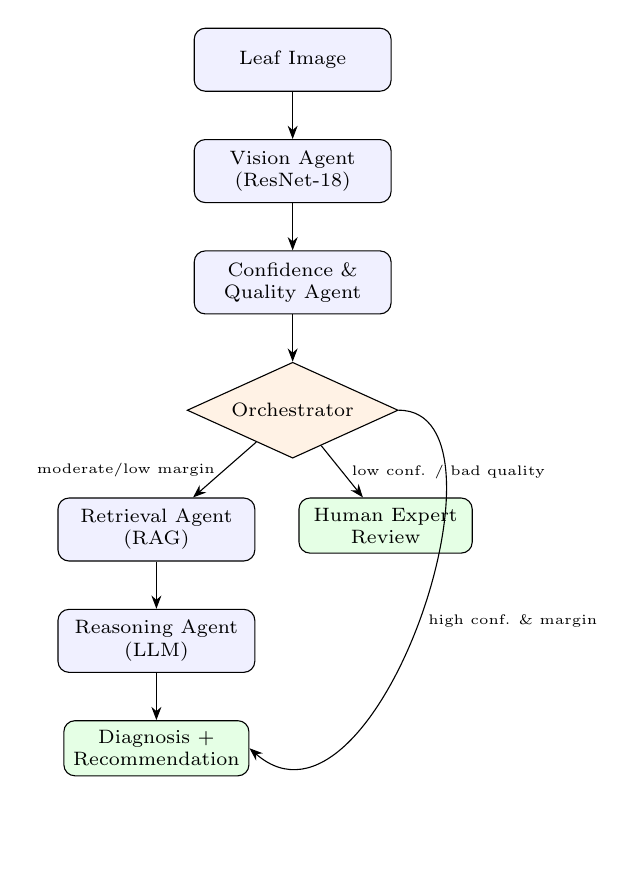
\begin{tikzpicture}[
  node distance=6mm and 8mm,
  box/.style={draw, rounded corners, minimum width=2.5cm, minimum height=0.8cm, align=center, font=\scriptsize, fill=blue!6},
  decision/.style={draw, diamond, aspect=2.2, minimum width=2.4cm, align=center, font=\scriptsize, fill=orange!10},
  term/.style={draw, rounded corners, minimum width=2.2cm, minimum height=0.7cm, align=center, font=\scriptsize, fill=green!10},
  arrow/.style={-Stealth, thin}
]
\node[box] (img) {Leaf Image};
\node[box, below=of img] (vision) {Vision Agent\\ (ResNet-18)};
\node[box, below=of vision] (conf) {Confidence \&\\ Quality Agent};
\node[decision, below=of conf] (orch) {Orchestrator};
\node[box, below left=8mm and -2mm of orch] (retrieval) {Retrieval Agent\\ (RAG)};
\node[box, below=of retrieval] (reason) {Reasoning Agent\\ (LLM)};
\node[term, below right=8mm and -6mm of orch] (human) {Human Expert\\ Review};
\node[term, below=of reason] (out) {Diagnosis +\\ Recommendation};

\draw[arrow] (img) -- (vision);
\draw[arrow] (vision) -- (conf);
\draw[arrow] (conf) -- (orch);
\draw[arrow] (orch) -- node[left, font=\tiny]{moderate/low margin} (retrieval);
\draw[arrow] (retrieval) -- (reason);
\draw[arrow] (reason) -- (out);
\draw[arrow] (orch) -- node[right, font=\tiny]{low conf. / bad quality} (human);
\draw[arrow] (orch.east) .. controls +(1.6,0) and +(1.6,-1.4) .. node[right, font=\tiny]{high conf. \& margin} (out.east);
\end{tikzpicture}
\caption{Proposed agentic architecture. The Orchestrator conditionally routes each case to a fast direct-answer path, the full retrieval-and-reasoning path, or human escalation.}
\label{fig:arch}
\end{figure}

\subsection{Vision Agent}
The Vision Agent maps an input leaf image to a probability distribution over the PlantVillage disease taxonomy using one or more ResNet-18 convolutional networks \cite{r_he2016}. The backbones are reused from our prior federated learning study on plant disease classification, in which they were trained across simulated clients under a non-IID partition of the training data. The system supports two configurations: a single ResNet-18, and an ensemble of three ResNet-18 checkpoints produced by distinct federated aggregation strategies -- Federated Averaging (FedAvg), Federated Optimization (FedOpt), and Federated Matched Averaging (FedMA) -- whose softmax distributions are averaged. The ensemble additionally yields an \emph{agreement ratio}: the fraction of member models whose individual top-1 prediction matches the averaged ensemble label. This serves as a model-based uncertainty signal complementary to the softmax confidence, since independently trained models can diverge on a hard case even when the averaged confidence is high. In the present system the Vision Agent is used purely as a perception module: it emits the predicted label, the full class-probability distribution, and -- in ensemble mode -- the agreement ratio, all of which are passed to the next agent.

\subsection{Confidence and Image-Quality Agent}
This agent performs lightweight, non-parametric post-processing on the Vision Agent's output and on the input image itself, producing a structured reliability signal rather than a new prediction. Up to four quantities are computed: (i) \emph{confidence}, the top-1 softmax probability; (ii) \emph{margin}, the gap between the top-1 and top-2 class probabilities, which captures ambiguity between visually similar diseases that raw confidence alone can miss; (iii) a binary \emph{quality flag}, derived from a Laplacian-variance blur check and a brightness-range check on the input image, to catch cases where the image itself -- rather than the disease -- is the source of uncertainty; and (iv) when the Vision Agent runs as an ensemble, the \emph{agreement ratio} propagated from it, which flags cases where independently trained models disagree even if the averaged confidence is high. These signals are passed to the Orchestrator as a single structured object.

\subsection{Retrieval Agent}
The Retrieval Agent implements retrieval-augmented generation over a static knowledge base curated from publicly available agricultural extension and plant-pathology reference material, covering the crops and diseases represented in the PlantVillage taxonomy. Each reference document is embedded and indexed for dense semantic retrieval. Given a predicted disease label (and, when the margin is low, its runner-up candidate), the Retrieval Agent returns the top-$k$ most relevant passages, which serve as grounding evidence for the Reasoning Agent. This agent is invoked only when the Orchestrator determines that a case warrants full reasoning, rather than on every prediction.

\subsection{Reasoning Agent}
The Reasoning Agent is a large language model prompted with the predicted label, its confidence and margin, and the passages returned by the Retrieval Agent. It produces three outputs: (i) a diagnosis statement identifying the most likely disease and, when margin is low, up to two plausible alternatives; (ii) an explanation that is required to cite which retrieved passage supports each factual claim, so that the output can be checked for grounding rather than accepted as an unverifiable model assertion; and (iii) a treatment and prevention recommendation drawn from the retrieved evidence rather than generated from unverified parametric knowledge.

\subsection{Orchestrator}
The Orchestrator is the component that makes the system agentic rather than a fixed pipeline: it decides, per case, which of the other agents to invoke. Its policy is summarized in Table~\ref{tab:policy}. High-confidence, high-margin, good-quality cases bypass retrieval and reasoning entirely and are answered directly from a lookup, minimizing latency and inference cost. Moderate-confidence or low-margin cases trigger the full retrieval-and-reasoning pipeline. Low-confidence or low-quality cases are escalated directly to human review without any automated treatment recommendation being issued, since an automated system should not offer possibly harmful advice under conditions where it cannot support that advice. In ensemble mode, heavy disagreement among the member models (agreement ratio below a threshold) is treated as an additional escalation trigger, since divergence between independently trained models is itself evidence that the case is unreliable, even when the averaged softmax confidence is high.

\begin{table}[t]
\centering
\caption{Orchestrator Routing Policy}
\label{tab:policy}
\small
\begin{tabular}{p{3.6cm}p{3.6cm}}
\toprule
\textbf{Condition} & \textbf{Action} \\
\midrule
High confidence, high margin, model agreement, good image quality & Direct lookup-based recommendation; retrieval and reasoning skipped \\
Moderate confidence, or low margin, good image quality & Full pipeline: retrieval $\rightarrow$ reasoning $\rightarrow$ grounded recommendation with caveats \\
Low confidence, poor image quality, or heavy model disagreement & Escalate to human expert; no automated recommendation issued \\
\bottomrule
\end{tabular}
\end{table}

Algorithm~\ref{alg:orch} formalizes this routing logic.

\begin{algorithm}[t]
\caption{Orchestrator Routing Policy}
\label{alg:orch}
\begin{algorithmic}[1]
\REQUIRE image $x$; thresholds $\tau_{high}=0.85$, $\tau_{low}=0.55$, $\tau_{margin}=0.15$, $\tau_{agree}=0.5$
\STATE $\hat{y}, p, a \leftarrow \text{VisionAgent}(x)$ \COMMENT{label, softmax vector, agreement ratio}
\STATE $c \leftarrow \max(p)$; \ $m \leftarrow p_{(1)} - p_{(2)}$ \COMMENT{confidence, margin}
\STATE $q \leftarrow \text{QualityCheck}(x)$ \COMMENT{blur / brightness check}
\IF{$c \geq \tau_{high}$ \AND $m \geq \tau_{margin}$ \AND $a \geq \tau_{agree}$ \AND $q = \text{good}$}
    \STATE \textbf{return} DirectLookup($\hat{y}$) \COMMENT{skip retrieval \& reasoning}
\ELSIF{$c \geq \tau_{low}$ \AND $a \geq \tau_{agree}$ \AND $q = \text{good}$}
    \STATE $D \leftarrow \text{RetrievalAgent}(\hat{y})$
    \STATE \textbf{return} ReasoningAgent($\hat{y}, c, m, D$)
\ELSE
    \STATE \textbf{return} EscalateToHuman($x, \hat{y}, c, q, a$)
\ENDIF
\end{algorithmic}
\end{algorithm}

\subsection{Scope: Memory and Longitudinal Tracking}
An episodic Memory Agent that logs each diagnosis and a Follow-up Agent that requests a subsequent image to track disease progression over time are natural extensions of this architecture, consistent with the long-term and episodic memory categories discussed in Section~\ref{sec:related}. We deliberately scope them out of the present implementation, both because they require longitudinal image data not available in the PlantVillage benchmark and to keep the system within a tractable, rigorously evaluable footprint; they are discussed further as future work in Section~\ref{sec:conclusion}.

\section{Implementation Details}
\label{sec:impl}

\textbf{Dataset.} We use the PlantVillage dataset \cite{r_hughes2015}, comprising leaf images spanning multiple crop species and disease categories, split into training, validation, and held-out test partitions consistent with our prior federated learning experiments on this dataset.

\textbf{Vision backbone.} ResNet-18 \cite{r_he2016} is reused unmodified from prior work; no retraining was performed for this study, isolating the evaluation to the contribution of the agentic layer. We evaluate two Vision Agent configurations: a single FedAvg-trained checkpoint, and a three-model ensemble that combines checkpoints trained with FedAvg, FedOpt, and FedMA aggregation by averaging their softmax outputs. All three checkpoints share the same 38-class ResNet-18 architecture and differ only in their federated aggregation strategy.

\textbf{Orchestrator thresholds.} The high-confidence, low-confidence, and margin thresholds are configured at 0.85, 0.55, and 0.15 respectively; in ensemble mode, an agreement-ratio threshold of 0.5 additionally escalates cases on which the member models substantially disagree. The thresholds are selected to bias the system toward caution: cases are escalated rather than acted upon whenever confidence, margin, or inter-model agreement falls outside a conservative operating range.

\textbf{Retrieval index.} Reference documents are chunked and embedded with the \texttt{bge-small-en-v1.5} sentence-embedding model and indexed in a FAISS vector store for cosine-similarity retrieval; the Retrieval Agent returns the top-$k$ ($k=5$) passages per query.

\textbf{Reasoning model.} The Reasoning Agent is implemented with an instruction-tuned large language model accessed through an OpenAI-compatible API via a provider-agnostic wrapper, so that the model can be swapped without changing the rest of the system. It is prompted with a fixed template requiring passage-grounded citation for every factual claim in its output and instructed to decline to recommend a treatment that the retrieved evidence does not support.

\textbf{Knowledge base.} The static reference corpus underlying the Retrieval Agent comprises 125 curated documents drawn from open-access PubMed Central articles and agricultural extension / plant-pathology reference material, covering symptoms, causal pathogens, and management practices for the crop-disease categories present in the PlantVillage taxonomy. Chunking and embedding each document independently yields 16{,}706 indexed passage chunks, allowing the Retrieval Agent to return passage-level rather than document-level evidence to the Reasoning Agent.

\textbf{Episodic logging.} Every case processed by the Orchestrator, together with its routing decision and downstream output, is logged in a structured record. This log is used for offline evaluation (Section~\ref{sec:exp}) and, as discussed in Section~\ref{sec:conclusion}, forms the basis on which a full episodic Memory Agent could be built in future work.

\section{Experimental Setup}
\label{sec:exp}

We evaluate the system on a held-out PlantVillage test set of 114 images (three per class across all 38 crop-disease categories), reporting results for both the single-model and the three-model ensemble Vision Agent configurations, using two families of metrics.

\textbf{Classification metrics.} Top-1 accuracy and macro-averaged F1 score of the Vision Agent in isolation, to establish the baseline perceptual performance the agentic layer builds upon.

\textbf{Agentic metrics.} For each test case, let the system's action be either \emph{act} (issue a treatment recommendation, whether via the direct-lookup or full-reasoning path) or \emph{escalate} (defer to a human). We define:
\begin{align}
\text{Correct-action rate} &= \frac{|\{\,\text{act} \wedge \hat{y}=y\,\}|}{N} \\
\text{Harmful-action rate} &= \frac{|\{\,\text{act} \wedge \hat{y}\neq y\,\}|}{N} \\
\text{Human-intervention rate} &= \frac{|\{\,\text{escalate}\,\}|}{N}
\end{align}
where $\hat{y}$ is the predicted label, $y$ is the ground-truth label, and $N$ is the number of test cases. We additionally report the \emph{naive baseline harmful-action rate}, defined as the classifier's raw error rate under a policy that always acts regardless of confidence -- equivalent to deploying the Vision Agent alone without any orchestration. The reduction from this baseline to the agentic harmful-action rate is the primary indicator of the value added by the Confidence/Quality Agent and Orchestrator.

\textbf{Grounding check.} On the reasoning outputs from cases routed through the full pipeline, we qualitatively inspect whether cited factual claims are supported by the retrieved passages they reference and whether the agent declines to recommend treatments that the evidence does not contain. A formal, large-scale grounding annotation with inter-annotator agreement is left to future work.

\textbf{Retrieval coverage.} We additionally measure retrieval coverage as the fraction of the 38 classes for which the knowledge base returns at least one strongly relevant passage (cosine similarity $\geq 0.75$) when queried by class name.

\section{Results and Discussion}
\label{sec:results}

Table~\ref{tab:results} reports classifier and agentic-pipeline performance on the PlantVillage test set for both Vision Agent configurations.

\begin{table}[t]
\centering
\caption{Classification and Agentic Pipeline Results (114-image test set). Starred ensemble values are optimistic; see Section~\ref{sec:results} Limitations.}
\label{tab:results}
\small
\begin{tabular}{lcc}
\toprule
\textbf{Metric} & \textbf{Single} & \textbf{3-Model} \\
 & \textbf{ResNet-18} & \textbf{Ensemble} \\
\midrule
Top-1 accuracy & 86.0\% & 100.0\%$^{*}$ \\
Macro-F1 & 82.8\% & 100.0\%$^{*}$ \\
Correct-action rate & 87.7\% & 97.4\% \\
Harmful-action rate & 3.5\% & 0.0\% \\
Naive baseline harmful-action rate & 14.0\% & 0.0\%$^{*}$ \\
Human-intervention rate & 17.5\% & 2.6\% \\
Direct-diagnosis rate & 65.8\% & 74.6\% \\
Full-pipeline (retrieve+reason) rate & 16.7\% & 22.8\% \\
Member-model disagreements & --\,($N{=}1$) & 21/114 \\
Retrieval coverage (of 38 classes) & 100\% & 100\% \\
\bottomrule
\end{tabular}
\end{table}

\textbf{Safety-coverage trade-off (single model).} With the single ResNet-18 backbone, the Vision Agent achieves a top-1 accuracy of 86.0\% and a macro-F1 of 82.8\%. Under the naive baseline policy, in which every prediction is acted upon regardless of confidence, the harmful-action rate is 14.0\%: in that fraction of cases the system would recommend a treatment despite an incorrect diagnosis. The full agentic pipeline reduces this to 3.5\% -- roughly a four-fold reduction -- at a human-intervention rate of 17.5\%. This confirms the intended safety-coverage trade-off described in Section~\ref{sec:arch}: a modest fraction of cases deferred to a human in exchange for a substantial reduction in autonomously issued incorrect advice.

\textbf{Effect of ensembling.} Replacing the single backbone with the three-model federated ensemble raises top-1 accuracy to 100\% on this test set and lifts the correct-action rate to 97.4\% while lowering the human-intervention rate to 2.6\%. The ensemble corrects several classes that the single model misclassified outright, and its members disagreed on 21 of the 114 images; this disagreement feeds the Orchestrator's escalation signal even where the averaged confidence is high. As noted below, however, the near-perfect accuracy in this configuration also saturates the safety comparison and should be read with caution.

\textbf{Grounding and coverage.} Retrieval coverage is complete: all 38 classes return strongly relevant passages from the knowledge base. Qualitative inspection of the full-pipeline reasoning outputs found that they cite specific retrieved passages for their factual claims and, when the retrieved evidence described symptoms but lacked management guidance, the Reasoning Agent declined to fabricate a treatment and instead recommended expert consultation -- the intended hallucination-averse behavior. Because the Orchestrator invokes the Retrieval and Reasoning Agents only for the subset of cases not resolved by the direct-lookup path, the full pipeline also incurs substantially lower average inference cost than a fixed design that always invokes retrieval and reasoning, though a full latency comparison is left for future work.

\subsection{Limitations}
Four limitations qualify the conclusions of this study. First, and most importantly, the reported accuracies -- particularly the 100\% attained by the ensemble -- reflect in-distribution recognition rather than field generalization. The test images are drawn from the same PlantVillage distribution used to train the classifiers, so a degree of train--test overlap is likely, and the ensemble figures marked with an asterisk in Table~\ref{tab:results} should be read as an upper bound rather than an expected deployment accuracy. A direct consequence is that the ensemble's naive-baseline harmful-action rate collapses to 0\%, which \emph{saturates} the safety comparison; the informative safety result is therefore the single-model configuration (14.0\% $\rightarrow$ 3.5\%), where the classifier makes genuine errors for the agentic layer to catch. A rigorous assessment would use out-of-distribution test data -- for example field-captured smartphone images or a distinct dataset such as PlantDoc -- and a larger, class-balanced test set than the three-images-per-class used here. Second, PlantVillage images are captured under controlled, largely uniform backgrounds, a well-documented gap relative to field-captured images with cluttered backgrounds and variable lighting; the Confidence and Image-Quality Agent partially mitigates this at inference time but was not evaluated on out-of-distribution field imagery. Third, the static knowledge base covers the disease categories represented in PlantVillage but is not exhaustive of regional cultivars, co-occurring stress factors, or emerging pathogens, so the Retrieval Agent's grounding is only as complete as its underlying corpus. Fourth, the Orchestrator's confidence, margin, and agreement thresholds were set conservatively by design rather than tuned against a validation objective; a learned or calibrated routing policy, noted in Section~\ref{sec:conclusion}, may achieve a more favorable safety-cost trade-off than the fixed thresholds used here.

\section{Conclusion and Future Work}
\label{sec:conclusion}

This paper presented an agentic AI framework that upgrades a standard CNN-based plant disease classifier into an autonomous, explainable, and safety-aware diagnostic advisory system. By decomposing the diagnostic process into a Vision Agent, a Confidence and Image-Quality Agent, a Retrieval Agent, a Reasoning Agent, and an Orchestrator that conditions computation and action on predictive uncertainty, the system moves beyond single-shot classification toward the autonomy, goal-directed reasoning, and environment-aware deferral that characterize agentic AI. The introduced agentic metrics -- correct-action rate, harmful-action rate, and human-intervention rate -- offer a more complete picture of deployment safety than classification accuracy alone, and our results demonstrate a substantial reduction in harmful autonomous actions relative to a naive always-act baseline.

Several extensions follow naturally from the architecture proposed here. An episodic \emph{Memory Agent} would allow the system to retain a history of diagnoses per field or farmer, enabling pattern detection across repeated visits. A \emph{Follow-up Agent} could request a subsequent image after a fixed interval to track disease progression or treatment efficacy over time, an evaluation that PlantVillage's single-image structure does not currently support and would require new longitudinal data collection. Finally, replacing the Orchestrator's fixed confidence and margin thresholds with a learned routing policy, and extending the Vision Agent to the federated multi-client setting explored in our related work, represent promising directions for future research toward deployable, trustworthy agricultural AI.

\begin{thebibliography}{00}

\bibitem{b1} D.~B. Acharya, K.~Kuppan, and B.~Divya, ``Agentic AI: Autonomous intelligence for complex goals -- a comprehensive survey,'' \emph{IEEE Access}, 2025.

\bibitem{b2} A.~Bandi, B.~Kongari, R.~Naguru, S.~Pasnoor, and S.~V. Vilipala, ``The rise of agentic AI: A review of definitions, frameworks, architectures, applications, evaluation metrics, and challenges,'' \emph{Future Internet}, vol.~17, p.~404, 2025.

\bibitem{b3} F.~Binucci, P.~Banelli, P.~Di Lorenzo, and S.~Barbarossa, ``Dynamic resource allocation for multi-user goal-oriented communications at the wireless edge,'' in \emph{Proc. 30th European Signal Processing Conf. (EUSIPCO)}, 2022, pp.~697--701.

\bibitem{b4} U.~M. Borghoff, P.~Bottoni, and R.~Pareschi, ``Human-artificial interaction in the age of agentic AI: a system-theoretical approach,'' \emph{Frontiers in Human Dynamics}, vol.~7, p.~1579166, 2025.

\bibitem{b5} C.~Chawla, S.~Chatterjee, S.~S. Gadadinni, P.~Verma, and S.~Banerjee, ``Agentic AI: The building blocks of sophisticated AI business applications,'' \emph{Journal of AI, Robotics \& Workplace Automation}, vol.~3, pp.~1--15, 2024.

\bibitem{b6} S.~Hosseini and H.~Seilani, ``The role of agentic AI in shaping a smart future: A systematic review,'' \emph{Array}, p.~100399, 2025.

\bibitem{b9} A.~Kaplan and M.~Haenlein, ``Siri, Siri, in my hand: Who's the fairest in the land? On the interpretations, illustrations, and implications of artificial intelligence,'' \emph{Business Horizons}, vol.~62, pp.~15--25, 2019.

\bibitem{b10} Z.~Lin \emph{et al.}, ``Open source AI-based SE tools: Opportunities and challenges of collaborative software learning,'' \emph{ACM Trans. Softw. Eng. Methodol.}, vol.~34, pp.~1--24, 2025.

\bibitem{r1} Y.~Matsuo, Y.~LeCun, M.~Sahani, D.~Precup, D.~Silver, M.~Sugiyama, E.~Uchibe, and J.~Morimoto, ``Deep learning, reinforcement learning, and world models,'' \emph{Neural Networks}, vol.~152, pp.~267--275, 2022.

\bibitem{b13} S.~Murugesan, ``The rise of agentic AI: implications, concerns, and the path forward,'' \emph{IEEE Intelligent Systems}, vol.~40, pp.~8--14, 2025.

\bibitem{b12} S.~Sivakumar, ``Agentic AI in predictive AIOps: Enhancing IT autonomy and performance,'' \emph{Int. J. Scientific Research and Management}, vol.~12, pp.~1631--1638, 2024.

\bibitem{b14} Y.~Shavit \emph{et al.}, ``Practices for governing agentic AI systems,'' Research Paper, OpenAI, 2023.

\bibitem{r2} A.~Holzinger, G.~Langs, H.~Denk, K.~Zatloukal, and H.~M\"uller, ``Causability and explainability of artificial intelligence in medicine,'' \emph{WIREs Data Mining and Knowledge Discovery}, vol.~9, p.~e1312, 2019.

\bibitem{b11} N.~Karunanayake, ``Next-generation agentic AI for transforming healthcare,'' \emph{Informatics and Health}, vol.~2, pp.~73--83, 2025.

\bibitem{r_hughes2015} D.~P. Hughes and M.~Salath\'e, ``An open access repository of images on plant health to enable the development of mobile disease diagnostics,'' \emph{arXiv preprint arXiv:1511.08060}, 2015.

\bibitem{r_mohanty2016} S.~P. Mohanty, D.~P. Hughes, and M.~Salath\'e, ``Using deep learning for image-based plant disease detection,'' \emph{Frontiers in Plant Science}, vol.~7, p.~1419, 2016.

\bibitem{r_he2016} K.~He, X.~Zhang, S.~Ren, and J.~Sun, ``Deep residual learning for image recognition,'' in \emph{Proc. IEEE Conf. Computer Vision and Pattern Recognition (CVPR)}, 2016, pp.~770--778.

\bibitem{r_lewis2020} P.~Lewis \emph{et al.}, ``Retrieval-augmented generation for knowledge-intensive NLP tasks,'' in \emph{Advances in Neural Information Processing Systems (NeurIPS)}, 2020.

\end{thebibliography}

\end{document}